\begin{figure}[H]
	\centering
	\begin{tikzpicture}[node distance=1.5cm and 1cm, auto]
		% Nodo per immagine 2 con didascalia sotto, posizionato a destra di img1
		\node (img1) {
			\begin{tabular}{c}
				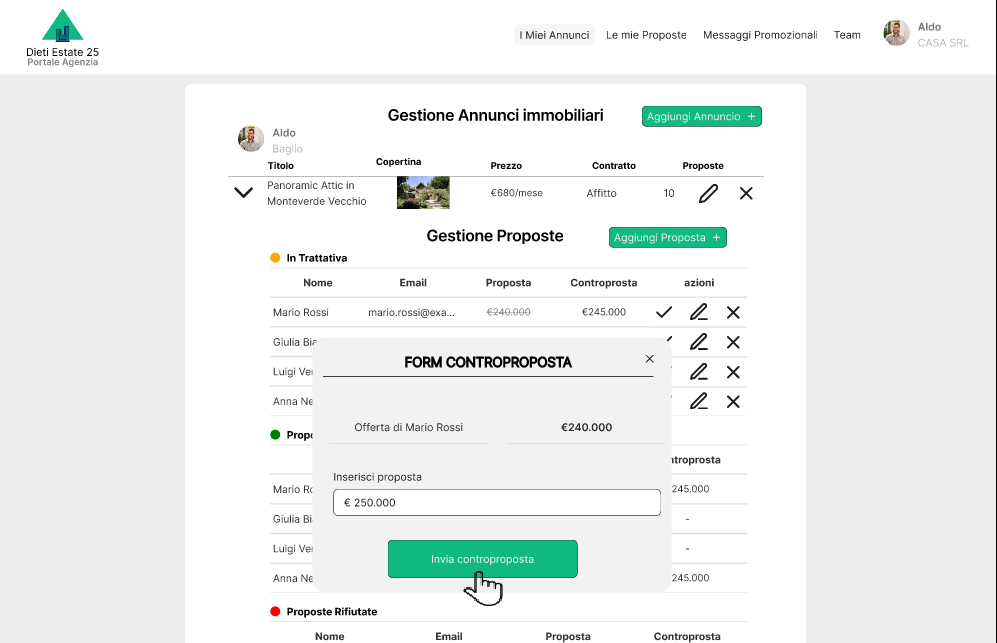
\includegraphics[width=0.7\textwidth]{Immagini/Mockup/controproposte/scenario principale/ClickInviaControproposta.png} \\
				Cockburn: step 6.A
			\end{tabular}
		};
		
		% Nodo per immagine 3 con didascalia sotto, posizionato sotto img2
		\node (img2) [below=of img1] {
			\begin{tabular}{c}
				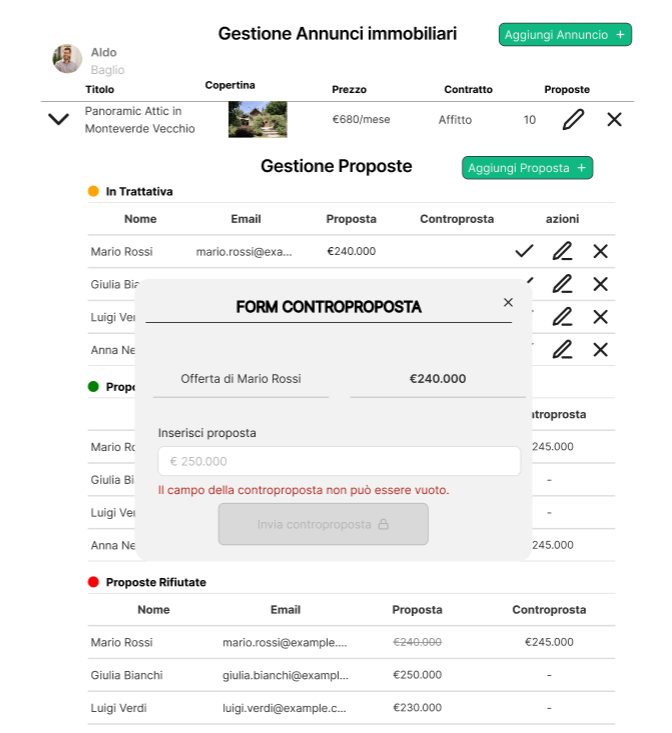
\includegraphics[width=0.7\textwidth]{Immagini/Mockup/controproposte/Extensions A/MessaggioDiErrore.png} \\
				Cockburn: step 7.A
			\end{tabular}
		};
		
		% Disegna le frecce
		\draw[->, thick] (img1) -- (img2);
		
	\end{tikzpicture}
	\caption{Mockup: Extension A della tabella di Cockburn del caso d'uso: Fare una controproposta a un'offerta.}
	\label{fig:tikz_flow}
\end{figure}

\newpage


